\chapter[Electromagnetic Calorimeters]{Electromagnetic Calorimeters
\footnote{
  $CVS~revision~ $Id: shower.tex,v 1.7 2005/04/04 22:27:25 gen Exp $ $
}
\footnote{Authors: E.Chudakov \email{gen@jlab.org}}
}
% This section written by P. Markowitz in Novermber 1996.
% V1.0 - OSP for PbG shower counters use
% Direct all comments/questions to:
% markowit@cebaf.gov
% TJNAF Room 16-116
% (757) 249 7237
% Updated:  April-18-1999 pecm included Armen's descriptions from web
% Rewritten by E.Chudakov  Dec,2003

\section{Purpose and Layout}

Electromagnetic calorimeters, or shower detectors, provide very good
particle identification (PID), separating electrons from hadrons or
muons \cite{Bartoszek:1991ex},\cite{Appel:1975tt}.  The electron's energy
is fully absorbed in a shower detector.  For a typical shower detector
thickness, about 20\% of hadrons pass through it without interaction,
releasing only the ionization energy.  The other 80\% interact
strongly in the detector. Still, many particles carrying a large
fraction of the initial energy escape from the detector. For
electromagnetic showers, the energy-release density peaks at a
detector depth of about 5 radiation lengths (the full detector depth
is about 20 radiation lengths), while the energy release of other
particles is more evenly distributed along the depth.  Therefore, two
factors are used for PID:
\begin{list}{\arabic{enumi}.~}{\usecounter{enumi}\setlength{\itemsep}{-0.15cm}}
  \item the ratio of the shower's energy to the particle's momentum;
  \item the longitudinal shower profile.
\end{list}

The HRS spectrometers are equipped with 2-layer segmented shower
detectors (see Fig.~\ref{fig:hrs-det-shower_layout}) built of
lead glass.
\begin{figure}[htb]
\begin{center}
   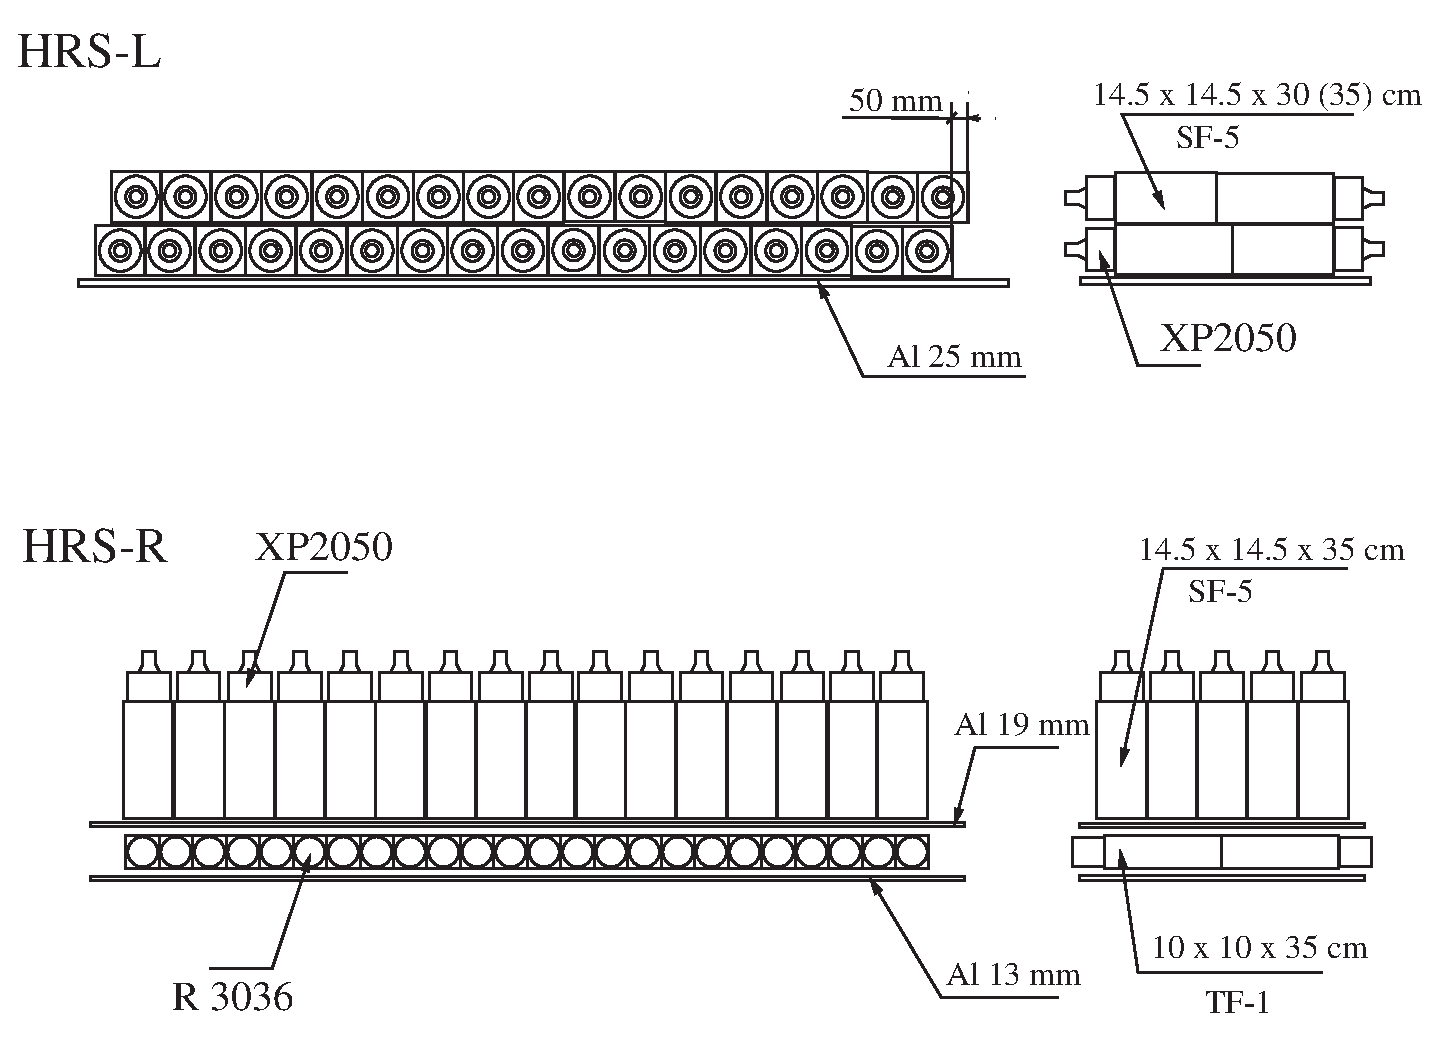
\includegraphics[angle=0,width=0.6\textwidth]{showerboth}
\end{center}
\caption[Schematic layout of part of the shower detectors in the HRS]%
{Schematic layout of part of the shower detectors in the HRS-L
(top) and HRS-R (bottom). Particles enter from the bottom of the figure.}
\label{fig:hrs-det-shower_layout}
\end{figure}
  
\infolevfour{
  A photo in Fig.~\ref{fig:hrs-det-presh-photo} shows the HRS-R
  first layer (``pre-shower'') detector installed, while the 
  second layer (``shower'') detector was removed.
\begin{figure}
\begin{center}
  \includegraphics[angle=0,width=0.6\textwidth]{hrs_det_preshower_2}
\end{center}
\caption[Detectors: Pre-shower Photo]{
  HRS-R 
  first layer (``pre-shower'') detector installed, while the 
  second layer (``shower'') detector was removed.
   }
\label{fig:hrs-det-presh-photo}
\end{figure}
} %infolev

The particle identification parameter
$R_{sh}$ is defined in Eq.~\ref{eq:shower-pid} as:

\begin{equation}
   R_{sh} = {E_{tot}\over{p}} \times {\ln(E_{presh})\over{\ln(E_{ave})}}
   \label{eq:shower-pid}
\end{equation}

where $E_{tot}$ is the total energy deposited in the shower detector, 
$p$ the particle's momentum, $E_{presh}$ the energy deposited in the 
front layer and $E_{ave}$ the average energy deposited by an electron 
with momentum $p$. 

\infolevone{
\section{Description of Components}
\subsection{Detectors}

The detector components are summarized in Table~\ref{tab:shower-blocks}.
\begin{table}[htb]
\begin{center}
\begin{tabular}{|r|r|r|r|r|r|r|r|r|r|c|} \hline
  HRS  &  layer  &  historic         & number & cols$\times$rows & \multicolumn{3}{c|}{Sizes, cm} & glass & \multicolumn{2}{c|}{PM} \\
  \cline{5-7} \cline{9-10}
       &         &  name             & of blocks  &  &  X &  Y &  Z  &     & \multicolumn{1}{c|}{type}   & od, in \\  
\hline
  L    &  1      & pion rejector 1   & 34  & 2$\times$17 & 14.7 & 35.0 & 14.7  & SF5 & XP2050$^{(a)}$ & 5 \\    
  L    &  2      & pion rejector 2   & 34  & 2$\times$17 & 14.7 & 35.0 & 14.7  & SF5 & XP2050$^{(a)}$ & 5 \\    
  R    &  1      & pre-shower        & 48  & 2$\times$24 & 10.0 & 35.0 & 10.0  & TF1 &  R3036$^{(b)}$ & 3 \\    
  R    &  2      & shower (old)      & 80  & 5$\times$16 & 14.7 & 14.7 & 35.0    & SF5 & XP2050$^{(a)}$ & 5 \\    
  R    &  2      & shower            & 75  & 5$\times$15 & 15.0 & 15.0 & 32.5  & SF5 & XP3530B$^{(c)}$ & 5 \\    
\hline
\end{tabular}
\end{center}
\caption[Shower: detectors]{The number and sizes of the lead glass blocks
   used in the shower detectors of the HRS. ``X'' denotes the dispersive plane
   of the HRS, while ``Z'' is along the average particle direction,
   perpendicular to the focal plane. Some of the large blocks are 30~cm
   long, instead of 35~cm. The photo-multiplier tubes were from:
   (a) - Philips, now Photonis~\cite{PhotonisInd} (discontinued),
    and are gradually being replaced by (c) Photonis XP3530B~\cite{PhotonisInd};
   (b) - Hamamatsu~\cite{HamamatsuPM}, discontinued.
   }
\label{tab:shower-blocks}
\end{table}
Because of its reduced thickness, the resolution in 
the HRS-L is not as good as that of the shower detector in the HRS-R.

The High Voltage is controlled via EPICS~\cite{EPICSwww} and the 
Hall A MEDM~\cite{MEDMwww} (see Chapter \ref{chap:controls}).
The MEDM windows and the voltages are shown in Figs. \ref{fig:hrs-det-hv-hrsr-top},
\ref{fig:hrs-det-hv-hrsr-bot} and \ref{fig:hrs-det-hv-hrsl}.
\begin{figure}
\begin{center}
  \includegraphics[angle=0,width=0.98\textwidth]{medm_halla_hv_hrsr_top}
\end{center}
\caption[Detectors: Shower HRS-R HV top]{
  HRS-R: HV, ``top'' crate - includes the ``pre-shower''} 
\label{fig:hrs-det-hv-hrsr-top}
\end{figure}

\begin{figure}
\begin{center}
  \includegraphics[angle=0,width=0.98\textwidth]{medm_halla_hv_hrsr_bot}
\end{center}
\caption[Detectors: Shower HRS-R HV top]{
  HRS-R: HV, ``bottom'' crate - includes the ``shower'' detector.} 
\label{fig:hrs-det-hv-hrsr-bot}
\end{figure}

\begin{figure}
\begin{center}
  \includegraphics[angle=0,width=0.98\textwidth]{medm_halla_hv_hrsl_1}
\end{center}
\caption[Detectors: Shower HRS-L HV]{
  HRS-L: HV, includes the ``pion rejector''.} 
\label{fig:hrs-det-hv-hrsl}
\end{figure}

\subsection{Electronics}

The signals from PM tubes XP2050 (see Table \ref{tab:shower-blocks})
are electronically amplified by a factor of $\sim$8. The other signals
are not amplified. All the signals
are delivered via the 1~$\mu$s delay lines to LeCroy ADC 1881M.

} %infolev

\begin{safetyen}{10}{10}
\section{Safety Assessment}
\end{safetyen}

% The HV increase must be done by an expert. \\
  
  Before handling the HV bases on the detector stack:
 \begin{list}{\arabic{enumi}.~}{\usecounter{enumi}\setlength{\itemsep}{-0.15cm}}
    \item Turn off the HV.
    \item Make sure the HV can not be turned on remotely - turn off the HV crate,
          or put it in the ``local'' mode using the key at the front panel of
          the crate.
        . In order to ensure that the crate HV would not be turned on one can 
          also turn off the power switch at the rear panel of the crate.
%          An equivalent of the ``lock out / tag out'' procedure 
%          may use the key on the front panel of the LeCroy 1458 power supply
%          mainframe.
 \end{list}


 Keep in mind that each $15\times{}15\times{}35$~cm$^3$ detector has a mass of 
 about 35~kg.

\begin{safetyen}{0}{0}
\section[Authorized  Personnel]{Authorized  Personnel}
\end{safetyen}

\begin{namestab}{tab:shower:personnel}{Shower detectors: authorized personnel}{%
      Electromagnetic calorimeters (shower detectors) : authorized personnel.}
  \EugeneChudakov{\em Contact}
  \BogdanWojtsekhowski{}
  \JackSegal{}
  \HakobVoskanyan{}
\end{namestab}


% ===========  CVS info
% $Header: /group/halla/analysis/cvs/tex/osp/src/hrs_det/shower.tex,v 1.7 2005/04/04 22:27:25 gen Exp $
% $Id: shower.tex,v 1.7 2005/04/04 22:27:25 gen Exp $
% $Author: gen $
% $Date: 2005/04/04 22:27:25 $
% $Name:  $
% $Locker:  $
% $Log: shower.tex,v $
% Revision 1.7  2005/04/04 22:27:25  gen
% Chnges after the review
%
% Revision 1.6  2003/12/17 03:59:49  gen
% authorized personnel tables unfied
%
% Revision 1.5  2003/12/13 06:23:38  gen
% Septum added. Name tables. Polishing
%
% Revision 1.4  2003/12/05 07:12:10  gen
% shower.tex modified. infolevel added. Polishing
%
% Revision 1.3  2003/06/06 17:00:27  gen
% Revision printout changed
%
% Revision 1.2  2003/06/05 23:30:01  gen
% Revision ID is printed in TeX
%
% Revision 1.1.1.1  2003/06/05 17:28:30  gen
% Imported from /home/gen/tex/OSP
%
%  Revision parameters to appear on the output
